\documentclass[../main.tex]{subfiles}

\begin{document}
    \subsection{Lab 2}
    Während dem Durchlauf des Experimentes des Lab 2, werden diverse Daten physikalische Vorgängen
    gesammelt. Diese Daten umfassen Ort und Geschwindigkeit, sowie kinetische und potentielle Energie.Nachfolgend werden alle Daten als Funktion der Zeit in der Abbildung~\ref{fig:ImpulsRomeoJulia} bis Abbildung~\ref{fig:Endgeschwindigkeit}
    aufgegliedert.
    \newline
    \newline
    In Abbildung~\ref{fig:ImpulsRomeoJulia} ist deutlich zu erkennen, wie Romeo
    während der Beschleunigungsphase in den ersten Sekunden an Impuls gewinnt. 
    Nach fünf Sekunden Gleitphase stösst Romeo auf die Feder, wodurch er abgebremst
    wird und Impuls verliert, bis er schliesslich bei null ankommt. Der Impuls wird
    jedoch in der gespannten Feder gespeichert und beim Entspannen der Feder wieder
    auf den Würfel übertragen. Dadurch hat der Würfel nach der Beschleunigungsphase 
    wieder den gleichen Impuls wie zuvor. Da der Gesamtimpuls erhalten bleibt, haben Romeo und Julia nun beide ein Impuls von 2 Ns. In Abbildung~\ref{fig:gesamtImpuls} sieht man die addierten Impulse und wie dies nach der Kollision in der Tat gleich bleibt.
    \begin{figure}[H]
        \begin{center}
            \centerline{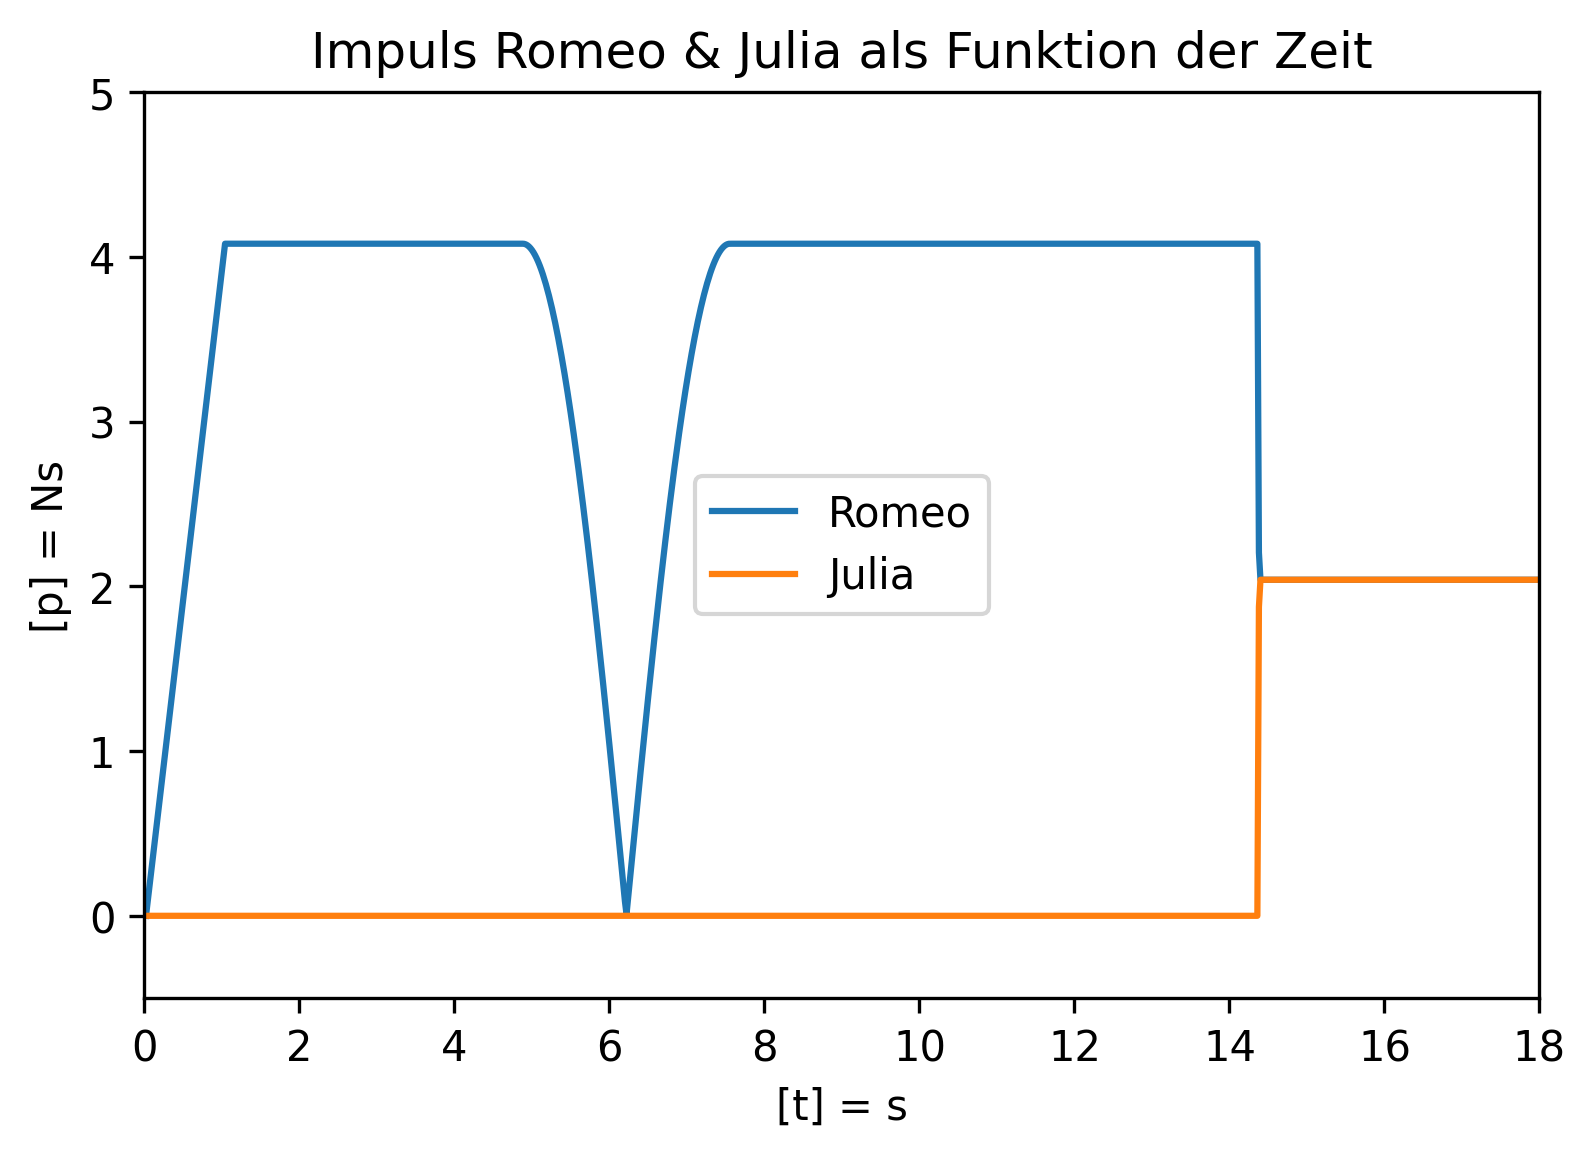
\includegraphics[width=105mm]{./images/Inelastisch/ImpulsRomeoJulia}}
            \caption{Impuls Romeo \& Julia als Funktion der Zeit}
            \label{fig:ImpulsRomeoJulia}
        \end{center}
    \end{figure}

    \begin{figure}[H]
        \begin{center}
            \centerline{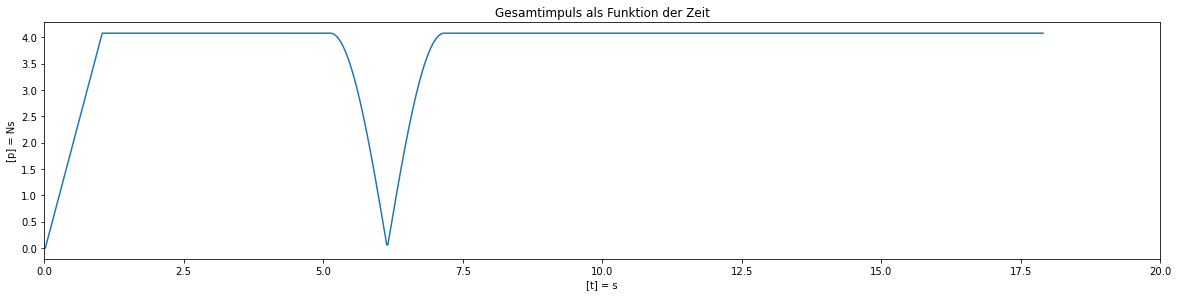
\includegraphics[width=105mm]{./images/Inelastisch/GesamtImpluls}}
            \caption{GesamtImpluls als Funktion der Zeit}
            \label{fig:gesamtImpuls}
        \end{center}
    \end{figure}

    \noindent    Im Ort-Zeit Diagramm in der Abbildung~\ref{fig:OrtRomeoJuliaAlsFunktionDerZeit} ist ersichtlich, dass Romeo bis Sekunde 5 sich bewegt und danach auf die Feder auftritt. Romeo bewegt sich dann gleichmässig in die entgegengesetze Richtung und nach 14 Sekunde ist zu sehen wie beide Würfel dann zusammen sich bewegen.
    \begin{figure}[H]
        \begin{center}
            \centerline{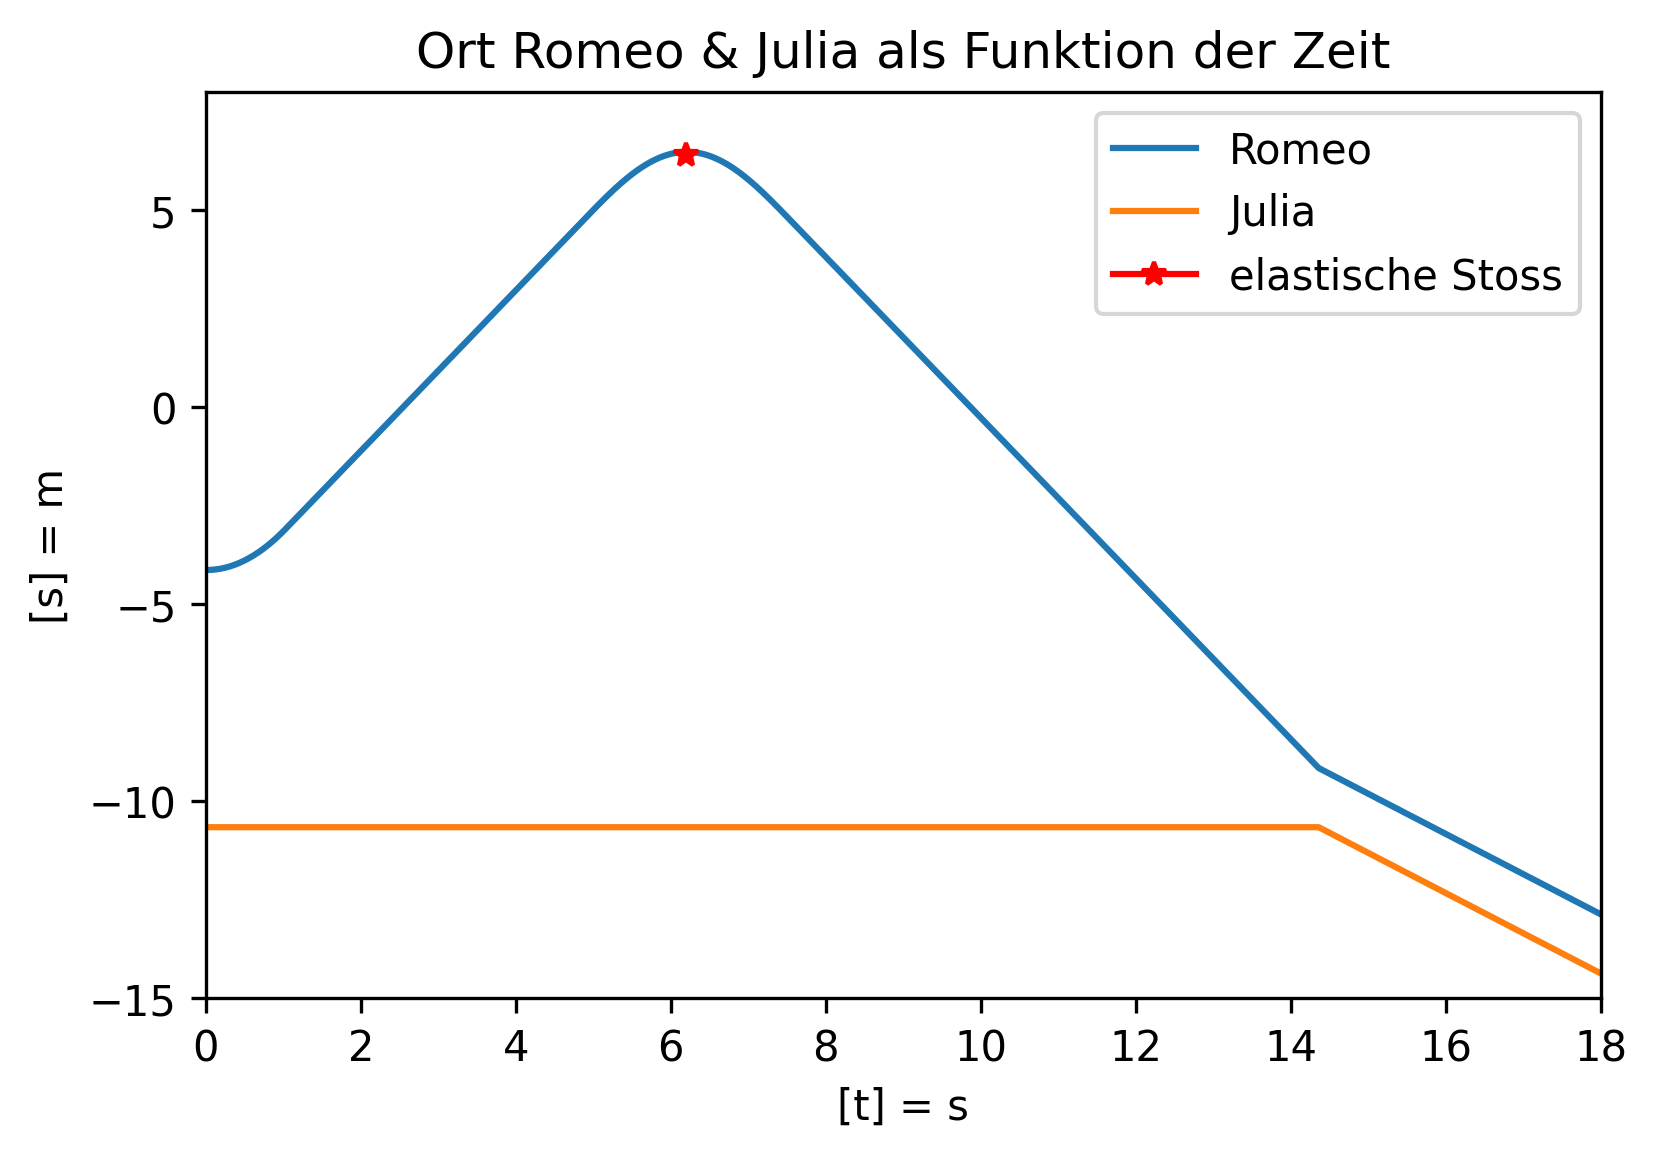
\includegraphics[width=105mm]{./images/Inelastisch/OrtRomeoJuliaAlsFunktionDerZeit}}
            \caption{Ort Romeo \& Julia als Funktion der Zeit}
            \label{fig:OrtRomeoJuliaAlsFunktionDerZeit}
        \end{center}
    \end{figure}

    \noindent    Gemäss Berechnung erreicht Romeo nach einer Sekunde die maximale Geschwindigkeit von 2 m/s und bewegt sich weiter mit dieser Geschwindigkeit bis es kurz vor Sekunde 6 auf die Feder trifft. Dann verändert sich wegen den Rüchstoss die Richtung der Geschwindigkeit. Beim inelastischen Stoss kleben Romeo und Julia zusammen und fahren mit der Schwerpunktgeschwindigkeit vEnde von 1 m/s, wie im Kapitel Physikalisch Beschreibung berechnet, weiter. In der Abbildung~\ref{fig:Endgeschwindigkeit} sieht man, dass dies in unseren Versuch auch übereinstimmt.
    \begin{figure}[H]
        \begin{center}
            \centerline{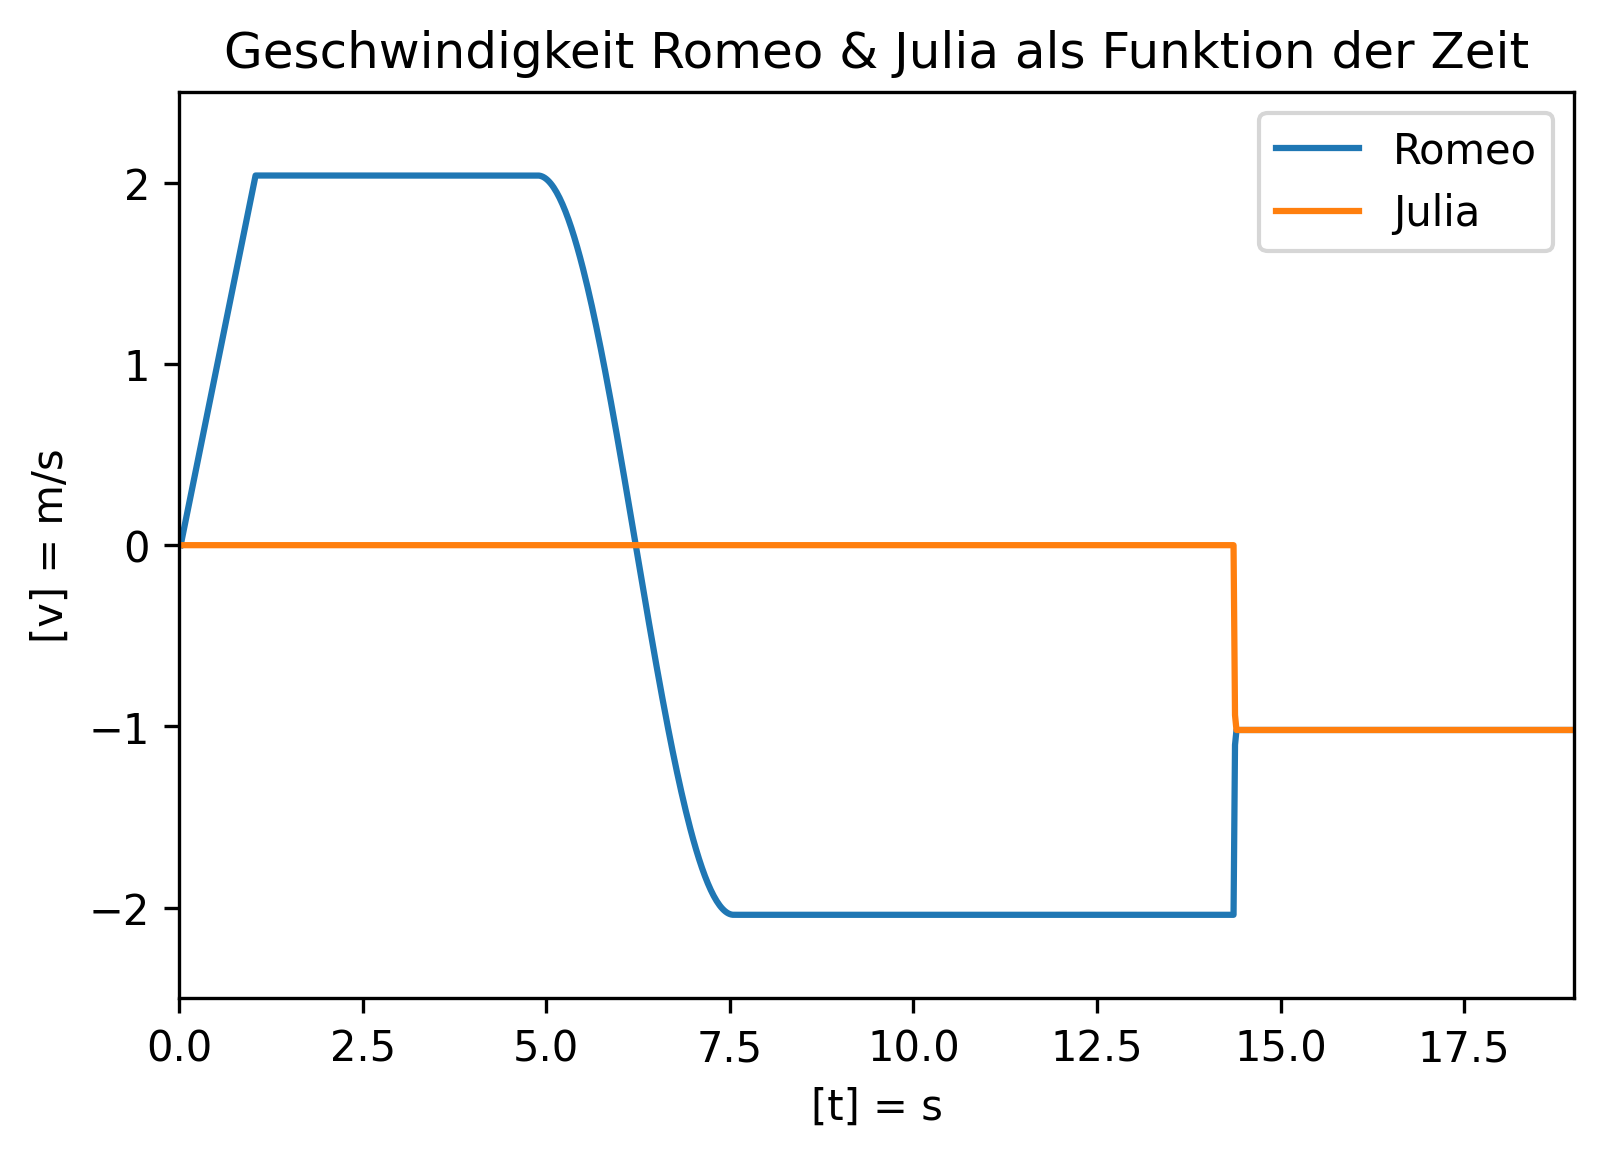
\includegraphics[width=105mm]{./images/Inelastisch/GeschwindigkeitRomeoJulia}}
            \caption{Geschwindigkeit Romeo \& Julia als Funktion der Zeit}
            \label{fig:GeschwindigkeitRomeoJulia}
        \end{center}
    \end{figure}

    \begin{figure}[H]
        \begin{center}
            \centerline{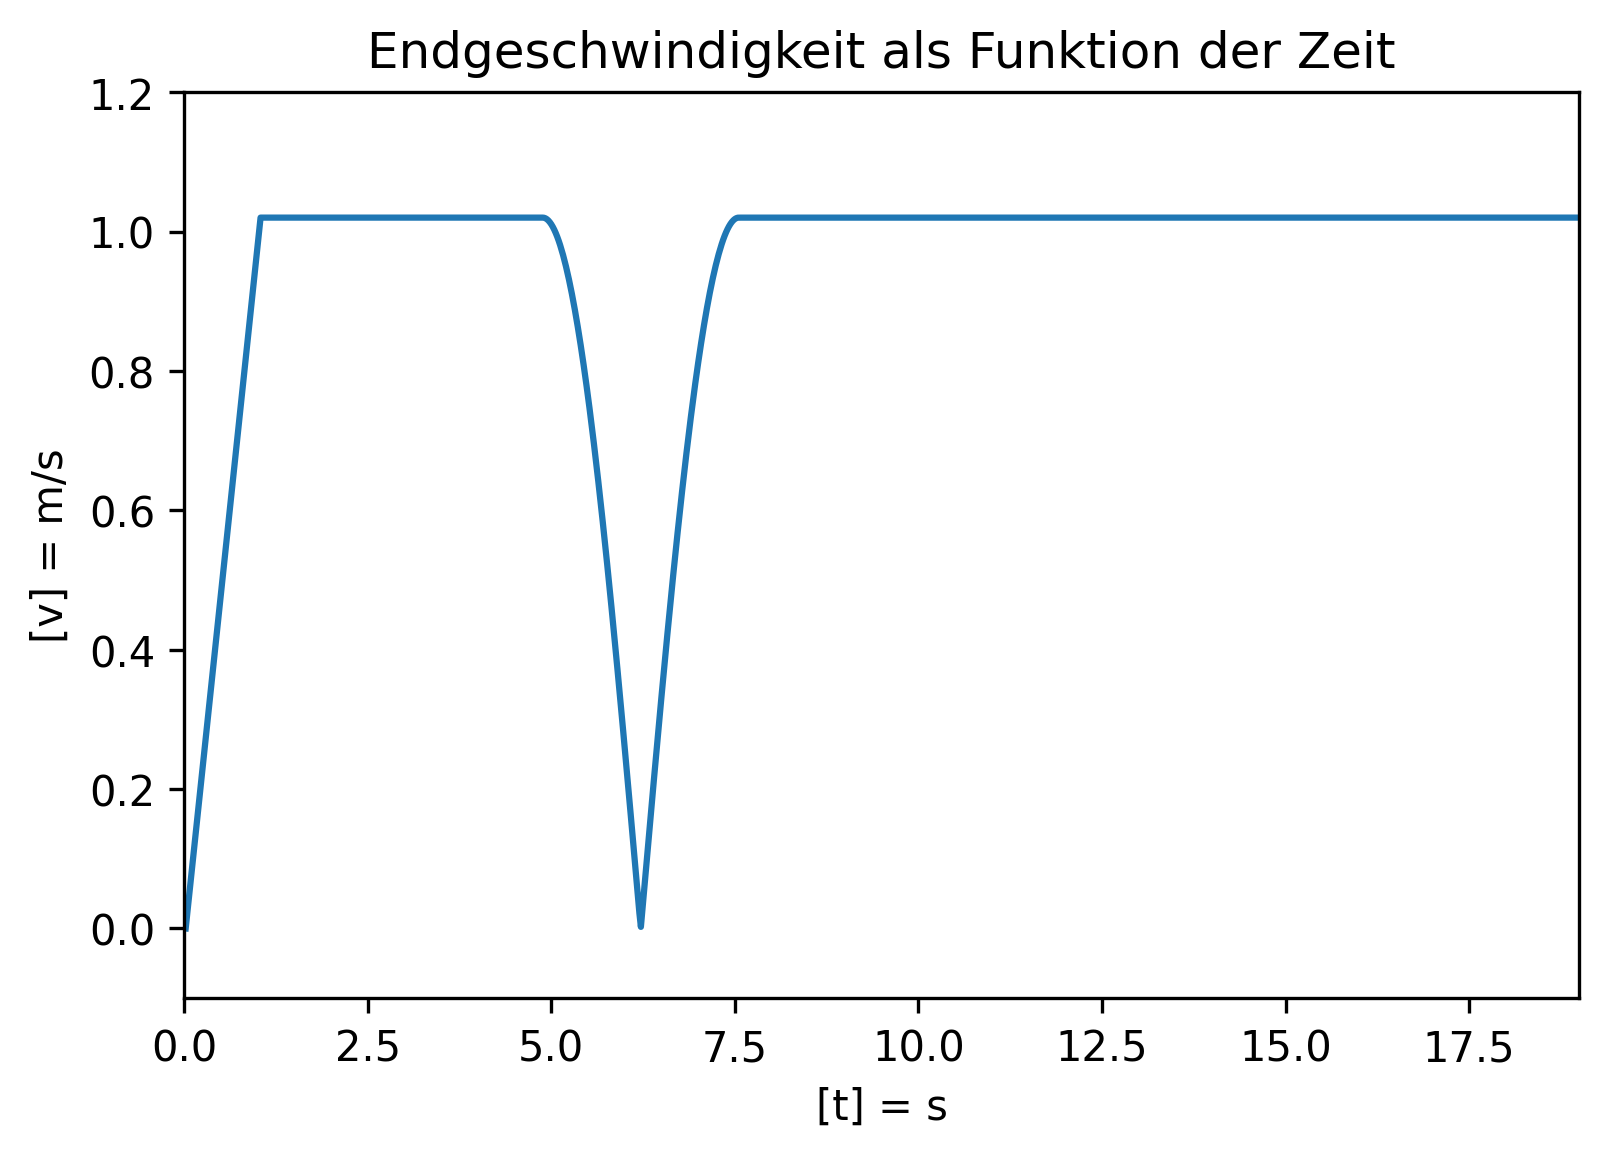
\includegraphics[width=105mm]{./images/Inelastisch/Endgeschwindigkeit}}
            \caption{Endgeschwindigkeit als Funktion der Zeit}
            \label{fig:Endgeschwindigkeit}
        \end{center}
    \end{figure}


    \subsection{Lab 3}

    \begin{figure}[H]
        \begin{center}
            \centerline{\includegraphics[width=105mm]{./images/ropeRomeo/Ortdiagramm}}
            \caption{Romeo Ortsdiagramm}
            \label{fig:RomeoOrtsdiagramm}
        \end{center}
    \end{figure}


    \begin{figure}[H]
        \begin{center}
            \centerline{\includegraphics[width=105mm]{./images/ropeRomeo/AuslenkungDeg}}
            \caption{Auslenkung Romeo in Grad als Funktion der Zeit}
            \label{fig:AuslenkungRomeo}
        \end{center}
    \end{figure}


    \begin{figure}[H]
        \begin{center}
            \centerline{\includegraphics[width=105mm]{./images/ropeJulia/Ortdiagramm}}
            \caption{Julia Ortsdiagramm}
            \label{fig:JuliaOrtsdiagramm}
        \end{center}
    \end{figure}


    \begin{figure}[H]
        \begin{center}
            \centerline{\includegraphics[width=105mm]{./images/ropeJulia/AuslenkungDeg}}
            \caption{Auslenkung Julia in Grad als Funktion der Zeit}
            \label{fig:AuslenkungJulia}
        \end{center}
    \end{figure}

\end{document}